\documentclass[tikz,border=4pt]{standalone}
\usepackage{amsmath,amssymb}\renewcommand{\familydefault}{\sfdefault}
\usepackage{pgfplots}\pgfplotsset{compat=1.17}
\usetikzlibrary{arrows.meta,positioning,shadows,fit,calc,backgrounds,patterns}
\definecolor{lav}{HTML}{E6E6FF}\definecolor{pinkb}{HTML}{FFDDDD}\definecolor{greenb}{HTML}{DDFFDD}\definecolor{yelb}{HTML}{FFFBCF}\definecolor{peach}{HTML}{FFEBD6}\definecolor{mauve}{HTML}{F0E6F0}
\definecolor{reqblue}{HTML}{0000BB}\definecolor{resgreen}{HTML}{008800}\definecolor{dred}{HTML}{CC0000}\definecolor{domblue}{HTML}{000099}\definecolor{crimson}{HTML}{990033}
\definecolor{tbBlue}{HTML}{1F77B4}\definecolor{tbOrange}{HTML}{FF7F0E}\definecolor{tbGreen}{HTML}{2CA02C}\definecolor{tbRed}{HTML}{D62728}\definecolor{tbPurple}{HTML}{9467BD}\definecolor{tbBrown}{HTML}{8C564B}
\definecolor{barGreen}{HTML}{1B8754}\definecolor{darkGreen}{HTML}{2E7D32}\definecolor{lightBlue}{HTML}{A0C4FF}\definecolor{kRed}{HTML}{DC3545}
\definecolor{accB}{HTML}{3366FF}\definecolor{f1O}{HTML}{FF7F50}\definecolor{aucG}{HTML}{44CC11}
\tikzset{node/.style={draw,rounded corners=2.5pt,thick,align=center},
 req/.style={-{Stealth[length=2.4mm]},thick,reqblue},res/.style={-{Stealth[length=2.4mm]},thick,dashed,resgreen}}
\pgfplotsset{every axis/.append style={tick label style={font=\footnotesize},label style={font=\small},title style={font=\small},legend style={font=\scriptsize,fill=white,fill opacity=.9,text opacity=1,draw=black!25,rounded corners=1pt},
 grid style={dotted,black!35}}}
\begin{document}
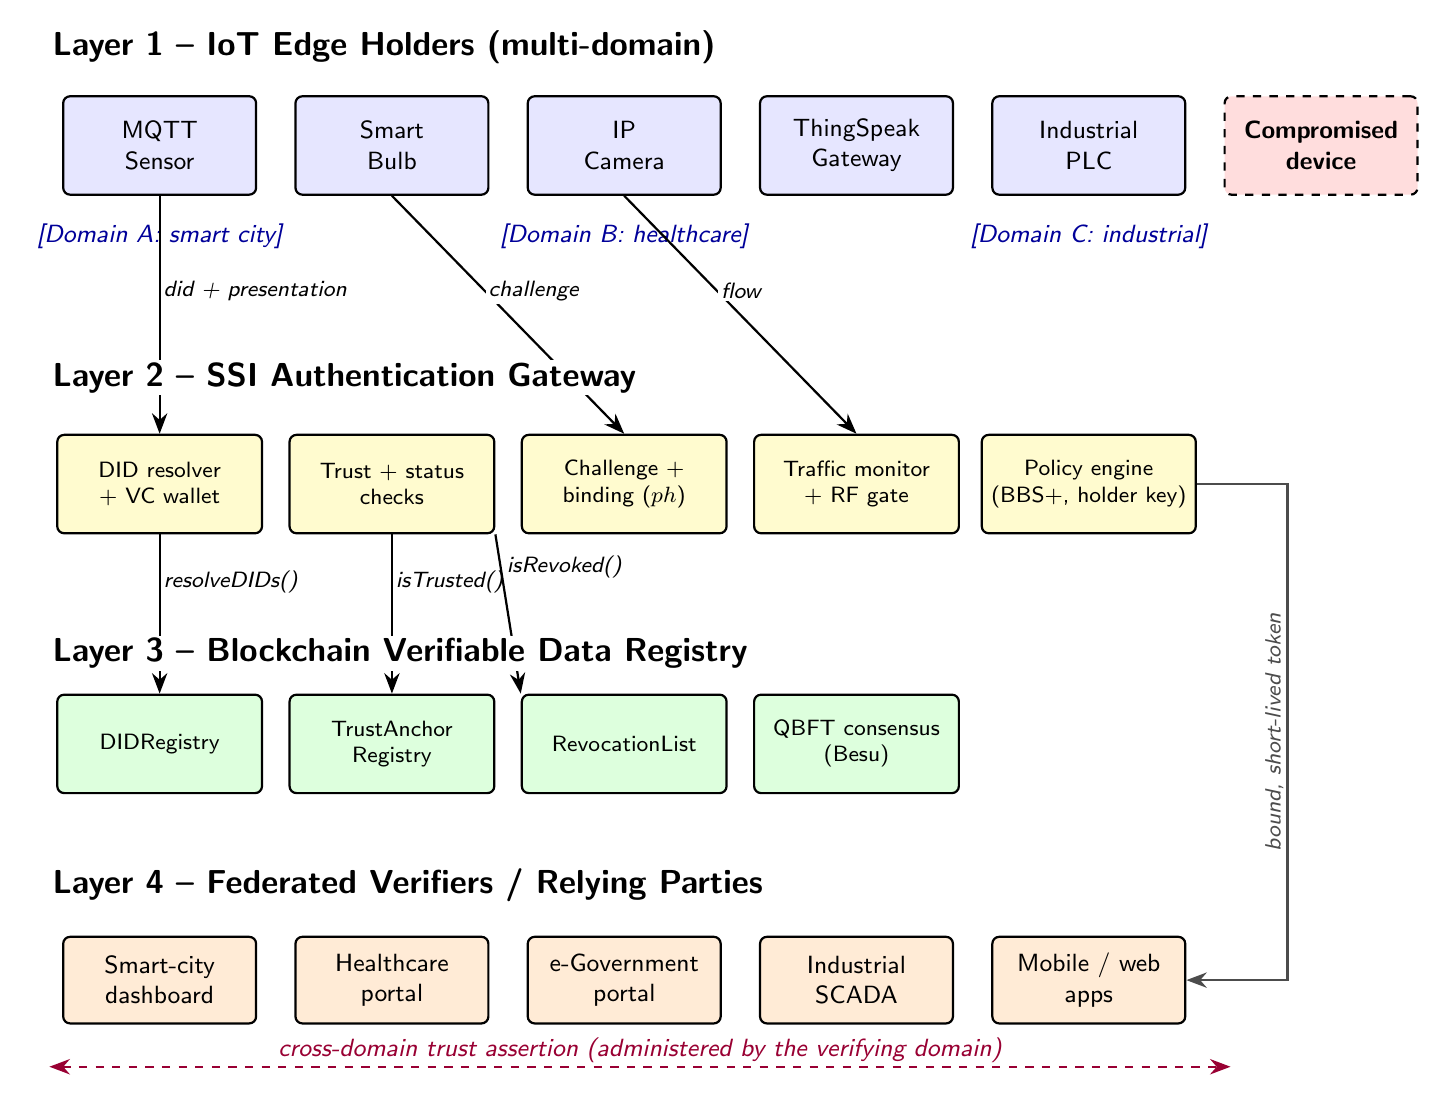
\begin{tikzpicture}[font=\small]
\tikzset{n1/.style={node,fill=lav,minimum width=2.45cm,minimum height=1.25cm,font=\small},n2/.style={node,fill=yelb,minimum width=2.6cm,minimum height=1.25cm,font=\footnotesize},
 n3/.style={node,fill=greenb,minimum width=2.6cm,minimum height=1.25cm,font=\footnotesize},n4/.style={node,fill=peach,minimum width=2.45cm,minimum height=1.1cm,font=\small},
 lbl/.style={font=\footnotesize\itshape,fill=white,inner sep=1pt}}
\node[n1] (d0) at (0.0,0) {MQTT\\Sensor};
\node[n1] (d1) at (2.95,0) {Smart\\Bulb};
\node[n1] (d2) at (5.9,0) {IP\\Camera};
\node[n1] (d3) at (8.850000000000001,0) {ThingSpeak\\Gateway};
\node[n1] (d4) at (11.8,0) {Industrial\\PLC};
\node[n1,fill=pinkb,dashed,font=\small\bfseries] (d5) at (14.75,0) {Compromised\\device};
\node[domblue,font=\small\itshape] at (0,-1.15) {[Domain A: smart city]}; \node[domblue,font=\small\itshape] at (5.9,-1.15) {[Domain B: healthcare]}; \node[domblue,font=\small\itshape] at (11.8,-1.15) {[Domain C: industrial]};
\node[n2] (g0) at (0.0,-4.3) {DID resolver\\+ VC wallet};
\node[n2] (g1) at (2.95,-4.3) {Trust + status\\checks};
\node[n2] (g2) at (5.9,-4.3) {Challenge +\\binding ($ph$)};
\node[n2] (g3) at (8.850000000000001,-4.3) {Traffic monitor\\+ RF gate};
\node[n2] (g4) at (11.8,-4.3) {Policy engine\\(BBS+, holder key)};
\node[n3] (r0) at (0.0,-7.6) {DIDRegistry};
\node[n3] (r1) at (2.95,-7.6) {TrustAnchor\\Registry};
\node[n3] (r2) at (5.9,-7.6) {RevocationList};
\node[n3] (r3) at (8.850000000000001,-7.6) {QBFT consensus\\(Besu)};
\node[n4] (v0) at (0.0,-10.6) {Smart-city\\dashboard};
\node[n4] (v1) at (2.95,-10.6) {Healthcare\\portal};
\node[n4] (v2) at (5.9,-10.6) {e-Government\\portal};
\node[n4] (v3) at (8.850000000000001,-10.6) {Industrial\\SCADA};
\node[n4] (v4) at (11.8,-10.6) {Mobile / web\\apps};
\draw[-{Stealth[length=2.6mm]},thick] (d0.south) -- (g0.north) node[pos=.4,right,lbl] {did + presentation};
\draw[-{Stealth[length=2.6mm]},thick] (d1.south) -- (g2.north) node[pos=.4,right,lbl] {challenge};
\draw[-{Stealth[length=2.6mm]},thick] (d2.south) -- (g3.north) node[pos=.4,right,lbl] {flow};
\draw[-{Stealth[length=2.6mm]},thick] (g0.south) -- (r0.north) node[pos=.3,right,lbl] {resolveDIDs()};
\draw[-{Stealth[length=2.6mm]},thick] (g1.south) -- (r1.north) node[pos=.3,right,lbl] {isTrusted()};
\draw[-{Stealth[length=2.6mm]},thick] (g1.south east) -- (r2.north west) node[pos=.3,above right,lbl] {isRevoked()};
\draw[-{Stealth[length=2.6mm]},thick,black!70] (g4.east) -- ++(1.15,0) |- (v4.east) node[pos=.25,above,rotate=90,lbl] {bound, short-lived token};
\draw[-{Stealth[length=2.6mm]},thick,dashed,crimson,thick,{Stealth[length=2.6mm]}-{Stealth[length=2.6mm]}] (-1.4,-11.7) -- (13.6,-11.7) node[midway,above,font=\small\itshape,crimson,fill=white,inner sep=1pt] {cross-domain trust assertion (administered by the verifying domain)};
\node[anchor=west,font=\large\bfseries,fill=white,inner sep=1pt] at (-1.4,1.25) {Layer 1 -- IoT Edge Holders (multi-domain)};
\node[anchor=west,font=\large\bfseries,fill=white,inner sep=1pt] at (-1.4,-2.95) {Layer 2 -- SSI Authentication Gateway};
\node[anchor=west,font=\large\bfseries,fill=white,inner sep=1pt] at (-1.4,-6.45) {Layer 3 -- Blockchain Verifiable Data Registry};
\node[anchor=west,font=\large\bfseries,fill=white,inner sep=1pt] at (-1.4,-9.4) {Layer 4 -- Federated Verifiers / Relying Parties};
\end{tikzpicture}
\end{document}
